% This file was created with tikzplotlib v0.9.15.
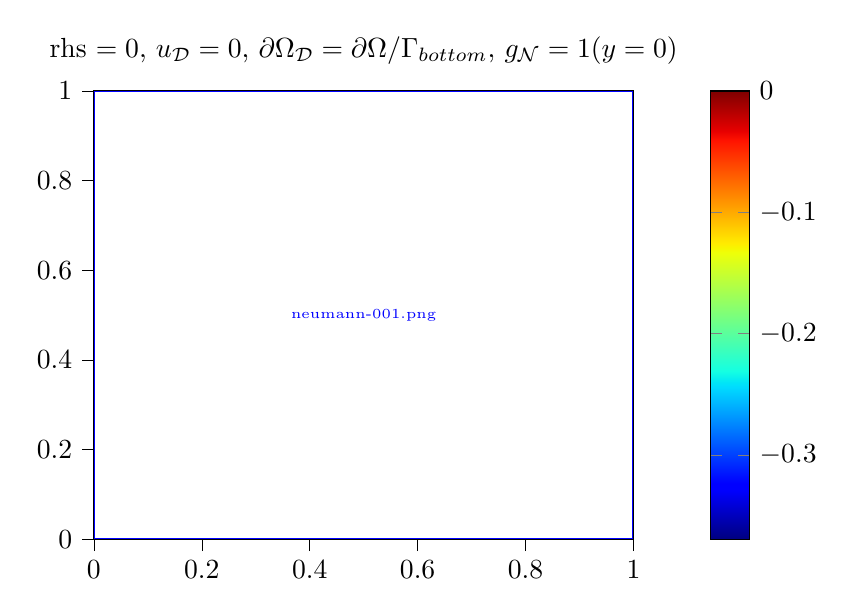
\begin{tikzpicture}

\begin{axis}[
colorbar,
colorbar style={ylabel={}},
colormap={mymap}{[1pt]
  rgb(0pt)=(0,0,0.5);
  rgb(22pt)=(0,0,1);
  rgb(25pt)=(0,0,1);
  rgb(68pt)=(0,0.86,1);
  rgb(70pt)=(0,0.9,0.967741935483871);
  rgb(75pt)=(0.0806451612903226,1,0.887096774193548);
  rgb(128pt)=(0.935483870967742,1,0.0322580645161291);
  rgb(130pt)=(0.967741935483871,0.962962962962963,0);
  rgb(132pt)=(1,0.925925925925926,0);
  rgb(178pt)=(1,0.0740740740740741,0);
  rgb(182pt)=(0.909090909090909,0,0);
  rgb(200pt)=(0.5,0,0)
},
point meta max=0,
point meta min=-0.369414712324147,
tick align=outside,
tick pos=left,
title={rhs \(\displaystyle =0\), \(\displaystyle u_\mathcal{D} = 0\), \(\displaystyle \partial\Omega_\mathcal{D}= \partial \Omega / \Gamma_{bottom} \), \(\displaystyle g_\mathcal{N} = 1(y=0)\)},
x grid style={white!69.0196078431373!black},
xmin=0, xmax=1,
xtick style={color=black},
y grid style={white!69.0196078431373!black},
ymin=0, ymax=1,
ytick style={color=black}
]
\addplot graphics [includegraphics cmd=\pgfimage,xmin=0, xmax=1, ymin=0, ymax=1] {neumann-001.png};
\end{axis}

\end{tikzpicture}
